\documentclass[a4paper]{article}

%% Useful packages
\usepackage{amsmath}
\usepackage{graphicx}	
\usepackage{algpseudocode}
\usepackage{algorithm}
\usepackage[colorinlistoftodos]{todonotes}
\usepackage[colorlinks=true, allcolors=black]{hyperref}
\usepackage[fontsize=11pt]{scrextend}
\usepackage{titlesec}
\usepackage[section]{placeins}
\usepackage{array}
\newcolumntype{L}[1]{>{\raggedright\let\newline\\\arraybackslash\hspace{0pt}}m{#1}}

\setlength\parindent{0pt}
\titleformat*{\section}{\Large\bfseries}
\titleformat*{\subsection}{\Large\bfseries}

\title{PowerEnjoy Service - Project Plan Document}

\begin{document}

\begin{titlepage}
\begin{figure}
\centering

\includegraphics[width=0.2\textwidth]{polimi.jpg}
\par
\LARGE Politecnico di Milano
\end{figure}


\maketitle
\textbf{Version 1.1}
\newline

\raggedright
Authors:
\begin{itemize}
	\item Domenico FAVARO (Mat. 837995)
        	\item Matheus FIM (Mat. 876069)
	\item Caio ZULIANI (Mat. 877266)	
\end{itemize}
\raggedleft
Prof. Elisabetta DI NITTO
\thispagestyle{empty}
\end{titlepage}

\tableofcontents
\newpage
 
\section{Introduction}
\subsection{Revision History}
This section records all revisions to the Document.
\newline \newline
\begin{tabular}{ | c | c | c | c | }
\hline
	Version & Date & Authors & Summary \\ \hline
	1.1 & 22/01/16 & Domenico Favaro, Caio Zuliani, Matheus Fim & Initial Release  \\ \hline
\end{tabular}

\subsection{Purpose and Scope}
The Project Plan Document (PPD) is fundamental to organize the production of the System. The main purpose of the Document is to study the complexity of the System, analize the difficulties that can be present in any stage of its development and deployment and give an overall estimation of the effort and cost that can be needed up to the final release of the product. The analysis will be done in terms of size, time and budget needed. This is fundamental to present our stakeholders a  preview before the start of production in case they need to do any project changing decision before hand.\par 
The second part of the Document helps the organization of our production by giving time estimations for each step and managing the workload of our resources accordingly. This serves our production team to make any project management decision but also our development team to know how they can organize themselves to follow the schedule and if by any reason the schedule can't be followed, they can notify the production. This is fundamental to keep track of the project developing at every stage of production.\par
Finally we present possible risks that can arise during the development and for each risk we have identified a contingency plan to avoid or minimize the possibility of harming the production.

\subsection{Definitions and Abbreviations}
\begin{itemize}
\item \textbf{RASD:} Reqirements And Specifications Document.
\item \textbf{DD:} Design Document.
\item \textbf{ITPD:} Integration Test Plan Document.
\item \textbf{PPD:} Project Plan Document
\item \textbf{App:} Application, refering to Web or Mobile App.
\item \textbf{LOC:} Lines of Code, is a software metric used to measure the size of a computer program by counting the number of lines in the text of the program's source code.
\item \textbf{FSM:} Functional Size Measurement, technique for measuring software in terms of the functionality it delivers.
\item \textbf{FP:} Function Points. Unit of measurement used to express the amount of functionality for an information system. We'll be using them to compute a FSM of software. 
\item \textbf{VAF:} Value Adjustment Factor, used to adjust the Function Points estimation to the context of the project.
\item \textbf{UFP:} Unadjusted Function Points, raw measurement of the total FP before the VAF is applied.
\item \textbf{ILF:} Internal Logic Files, FP Function Type.
\item \textbf{EIF:} External Interface Files, FP Function Type.
\item \textbf{EI:} External Input, FP Function Type.
\item \textbf{EO:} External Output, FP Function Type.
\item \textbf{EQ:} External Inquiries, FP Function Type.
\item \textbf{COCOMO:} Constructive Cost Model is a procedural software cost estimation model that we'll be using for this document.
\end{itemize}
For other concepts concerning the Service definition look in the \textbf{Glossary} section of the RASD, DD and ITPD.

\subsection{Reference Documents}
\begin{itemize}
\item Specification Document: Assignments AA 2016-2017.pdf
\item PowerEnjoy Requirements And Specifications Document (RASD)
\item PowerEnjoy Design Document (DD)
\item PowerEnjoy Integration Test Plan Document (ITPD)
\item Example Document - Project planning example document.pdf
\item Project Planning Tools Documentation:
\begin{itemize}
\item[-] Function Points Table
\begin{itemize}
	\item[-]\url{http://www.qsm.com/resources/function-point-languages-table}
\end{itemize}
\item[-] COCOMO II - Manual
\begin{itemize}
	\item[-]\href{http://csse.usc.edu/csse/research/COCOMOII/cocomo2000.0/CII_modelman2000.0.pdf}{COCOMO Model Definition Manual}
\end{itemize}
\item[-] Project Management Software: Jira/Trello
\begin{itemize}
	\item[-]\url{https://www.atlassian.com/software/jira}
	\item[-]\url{https://trello.com/}
\end{itemize}
\end{itemize}
\end{itemize}

\newpage
\section{Project Size, Cost and Effort Estimation}
This section deals with the estimation of the expected size, cost and effort needed to develop the PowerEnjoy Service.
For the size estimation we'll use the Function Points approach, once calculated we'll have an approximated size in LOC, and this measurement will be used later with COCOMO to predict the cost and amount of effort that will be required to develop the program.
\subsection{Size Estimation: Function Points}
The Function Mode approach is based in giving to each function needed in the code of the program a Category and a Complexity, once this is done, using Function Point Tables, a number of UFP is given to them. The VAF is then applied to the total of UFP. After the Total FP are calculated, it can then be translated into LOC.
The Categories for FP are 5, and each has its own rating table for complexity according to the number of Data Elements present:
\begin{itemize}
\item Internal Logic Files (ILF): \par
Translate to the sets of data used and managed by the application. 
\item External Interface Files (EIF): \par
Similar to ILF set of data used by the application but generated and maintained by other applications.\par
Their complexity table is the same as ILF.
\begin{center}
\begin{tabular}{ | c | c | c | c | }
\hline
	\textbf{Record Types} & \textbf{1-5} & \textbf{6-19} & \textbf{\(>\) 19}  \\ \hline\hline
	0-1 & Low & Low & Avg  \\ \hline
	2-3 & Low & Avg & High  \\ \hline
	\(>\) 3 & Avg & High & High  \\ \hline
\end{tabular}
\end{center}
\item External Inputs (EI): \par
Defined as operations to receive and manage data coming from the external environment.
\begin{center}
\begin{tabular}{ | c | c | c | c | }
\hline
	\textbf{File Types} & \textbf{1-4} & \textbf{5-15} & \textbf{\(>\)15} \\ \hline\hline
	0-1 & Low & Low & Avg  \\ \hline
	2 & Low & Avg & High  \\ \hline
	\(>\) 2 & Avg & High & High  \\ \hline
\end{tabular}
\end{center}
\newpage
\item External Outputs (EO): \par
They are elementary operations that generates data for the external environment. It usually includes managing data from logic files
\item External Inquiries (EQ): \par
Operation that involves both input and output, managing the data themselves without significant intervation from logic files.\par
Their complexity table is the same as EO.
\begin{center}
\begin{tabular}{ | c | c | c | c | }
\hline
	\textbf{File Types} & \textbf{1-5} & \textbf{6-19} & \textbf{\(>\)19} \\ \hline\hline
	0-1 & Low & Low & Avg  \\ \hline
	2-3 & Low & Avg & High  \\ \hline
	\(>\) 3 & Avg & High & High  \\ \hline
\end{tabular}
\end{center}
\end{itemize}
To measure the complexity in FP, weights are given to each Function Type using the following table:
\begin{center}
\begin{tabular}{ | c | c | c | c | }
\hline
	\textbf{Function Type} & \textbf{Low} & \textbf{Avg} & \textbf{High} \\ \hline\hline
	ILF & 7 & 10 & 15  \\ \hline
	EIF & 5 & 7 & 10  \\ \hline
	EI & 3 & 4 & 6  \\ \hline
	EO & 4 & 5 & 7  \\ \hline
	EQ & 3 & 4 & 6  \\ \hline
\end{tabular}
\end{center}

\subsubsection{Internal Logic Files (ILF)}
The PowerEnjoy System is organized to store a number of information to provide its functionalities. This information corresponds to the Entities that compose the System and will be manage by the Entity Beans in the Controllers \textit{(see DD)}. The ILF will then correspond to managing the information of these entities, which are:
\begin{itemize}
\item Cars: Cars will be stored in the system DB and replicated by persistent entities in the JEE2 environment for managing their status. Their information include CarID, Location, Status, BatteryStatus, if it's PluggedIn and Number of Passengers. \par Car element count is 6 Fields.
\item Users: Users tuples will be added by the System in the DB as well for the Registration feature, their attributes include UserID, if it's LoggedIn, UserName, Password, Email, DriverLicense, PaymentInfo and Location. 
\par User count is 8 Fields.
\item CRM: Although not directly added by the System, the loggedIn status of the CRMs is important for the Chat feature. It stores their CRMID, Password, Name, Email and if it's LoggedIn. 
\par CRM count is 5 Fields.
\item Reservations: Will link Users with Cars and will have a status to know wether the reservation is active or not. Their attributes are ReservationID, UserID, CarID, Status, ReservationTime, PickUpTime.
\par Reservation elements count is 6 and references 2 Record Types.
\item Rides: Once the Reservation has been confirmed a Ride is created, it refers to the Reservation and it tracks the use of the Car. It has RideID, ReservationID, CarID, Status, StartTime, EndTime, LocationPath.
\par Ride count is 7 and references 2 Record Types.
\item Payments: When the Ride is finished it generates the Payment for the User to pay, it tracks the input made by the Car, Rides and Users and include also eventual Discounts and Extra Fees. It has PaymentID, RideID, TotalFee, PassengerDiscount, BatteryDiscount, PluggedInDiscount, LowBatteryFee, NoPlugNearFee.
\par Payment has 8 fields, references 1 Record Type.
\item User Reports: Tracks any fault in the Service by Users or Cars and are handled by CRMs. They have the following fields: UserReportID, UserID, CRMID, CarID, Description.
\par User Report has 5 fields, references 3 Record Types.
\item Locations: Although not managed by the System, the record of safe parking and plug in areas has to be kept and accessed by the LocationHelper. They have basic Info like LocationID, Latitude, Longitude, Type.
\par Locations have 4 fields.
\end{itemize}
\newpage
Using the Complexity Table for the ILF we obtain the following.
\begin{center}
\begin{tabular}{ | l | c | c | }
\hline
	\textbf{ILF} & \textbf{Complexity} & \textbf{FP} \\ \hline\hline
	Car Data & Low & 7 \\ \hline
	User Data & Low & 7  \\ \hline
	CRM Data & Low & 7  \\ \hline
	Reservations & Avg & 10  \\ \hline
	Rides & Avg & 10 \\ \hline
	Payments & Low & 7  \\ \hline
	User Reports & Low &  7  \\ \hline
	Locations & Low & 7  \\ \hline
\end{tabular}
\end{center}
The Total UFP for ILF is \textbf{62}.

\subsubsection{External Interface Files (EIF)}
Our only external data source comes from Google Maps API, that offers the map service. It's used by the Location Helper and by the User and CRM Interface Components. It'll be accessed to retrieve the map interface find directions and show the location of the User and the Cars, as well as to retrieve walking and driving distances. The response is given in JSON and it provides numerous fields, however it doesn't reference any record types so we count only the number of parameters the response gives us.
\begin{center}
\begin{tabular}{ | l | c | c | }
\hline
	\textbf{EIF} & \textbf{Complexity} & \textbf{FP} \\ \hline\hline
	API Map Retrieval & Avg & 10 \\ \hline
	Direction Retrieval & Low & 7 \\ \hline
\end{tabular}
\end{center}
This gives us that the UFP for EIF are\textbf{17}.

\subsubsection{External Inputs (EI)}
The Sytem relies on many interactions provided for the User to allow them the functionalities of the service, others involve or are shared by the CRM, we'll present all of them and give a complexity estimation for each one. They consist on a function activated by the User Input.\newline
\par
Shared:
\begin{itemize}
\item Login: Controls that the parameters are correct and logs in the User. Low Complexity.
\item Logout: Signs out the connected User. Low Complexity.
\item Reserve Car: Creates a new Reservation. It involves User, Car and Reservation. Complexity Average.
\item Cancel Reservation: Cancels already created Reservation, interacts just with User and Reservation. Complexity Low.
\end{itemize}
Users:
\begin{itemize}
\item Register: Creates a new User and inserts his/her data in the system, has many fields but concers only the User. Complexity is Low.
\item Confirm Reservation: Unlocks the Car and starts a new Ride. Average Complexity.
\item End Ride: Finishes current Ride and creates a new Payment. Complexity is Average.
\end{itemize}
CRM:
\begin{itemize}
\item Create User Report: Links User, CRM and Car in case of any issue. Average Complexity.
\item Lock Car: Signals the Car to Lock. Low Complexity.
\item Unlock Car: Low Complexity.
\end{itemize}
\begin{center}
\begin{tabular}{ | l | c | c | }
\hline
	\textbf{EI} & \textbf{Complexity} & \textbf{FP} \\ \hline\hline
	Login & Low & 3 x2 \\ \hline
	Logout & Low & 3 x2 \\ \hline
	Register & Low & 3  \\ \hline
	Reserve Car & Avg & 4 x2  \\ \hline
	Cancel Reservation & Low & 3 x2 \\ \hline
	Confirm Reservation & Avg & 4 \\ \hline
	End Ride & Avg & 4 \\ \hline
	Create User Report & Avg &  4  \\ \hline
	Lock Car & Low & 3  \\ \hline
	Unlock Car & Low & 3  \\ \hline
\end{tabular}
\end{center}
This gives us a Total UFP for the EI of \textbf{47}.

\subsubsection{External Outputs (EO)}
PowerEnjoy External Outputs are limited to sending Emails in case of User Registration to send the password, End of Ride to send the Payment and Time Limit over the Reservation to notify the User.
\begin{itemize}
\item Email Password: Involves just the User, Low Complexity.
\item Email Payment: Sends Payment to User, Low Complexity.
\item Send Late Reservation Notification: Notifies status of Reservation to User, Low Complexity.
\end{itemize}
\begin{center}
\begin{tabular}{ | l | c | c | }
\hline
	\textbf{EO} & \textbf{Complexity} & \textbf{FP} \\ \hline\hline
	Notify Password & Low & 4 \\ \hline
	Notify Payment & Low & 4  \\ \hline
	Notify Reservation & Low & 4  \\ \hline
\end{tabular}
\end{center}
The Total UFP for the EO is \textbf{12}.

\subsubsection{External Inquiries (EQ)}
Similar to EI but sends a data response instead for the User. Basically a query of our system. PowerEnjoy EQ are:
\begin{itemize}
\item Search Nearby Cars: Gives a List of close by avaliable Cars from the User Location. Has Low Complexity.
\item Money Saving Option: Calculates the best Re-Charging station according to a standard Deviation Algorithm (\textit{see DD}) and returns it to the User so a discount for the ride can be applied. Is of Average Complexity.
\item Find Location: Gives a Path to arrive to the given Location.
\item Find Cars: Returns all desired Cars for the CRM.
\item Find Users: Returns all Users for the CRM.
\item Find Reservations: Returns desired Reservations for the CRM.
\item Find Rides: Returns all Rides for the CRM.
\item Find Payments: Returns given Payments for the CRM.
\item Find User Reports: Returns the User Reports for the CRM.
\end{itemize}
All the Finding Functions are considered to have Low Complexity.
\begin{center}
\begin{tabular}{ | l | c | c | }
\hline
	\textbf{EQ} & \textbf{Complexity} & \textbf{FP} \\ \hline\hline
	Search Nearby Cars & Low & 3 \\ \hline
	Money Saving Option & Avg & 4  \\ \hline
	Find Location & Low & 3  \\ \hline
	Find Cars & Low & 3  \\ \hline
	Find Users & Low & 3  \\ \hline
	Find Reservations & Low & 3  \\ \hline
	Find Rides & Low & 3 \\ \hline
	Find Payments & Low & 3 \\ \hline
	Find User Reports & Low &  3  \\ \hline
\end{tabular}
\end{center}
This gives us a Total UFP for the EQ of \textbf{28}.
\newpage

\subsubsection{Overall Estimation}
 The following table shows the estimation results for each Function Type:
\begin{center}
\begin{tabular}{ | c | c | }
\hline
	\textbf{Function Type} & \textbf{Value}\\ \hline\hline
	ILF & 62 \\ \hline
	EIF & 17 \\ \hline
	EI & 47 \\ \hline
	EO & 12 \\ \hline
	EQ & 28 \\ \hline
\end{tabular}
\end{center}
The added Total of UFP is \textbf{166}.\newline
\par
To have an idea of the size of our project in the code we translate the total of UFP to LOC using the Function Points Languages Table. Since we'll develop in the J2EE platform the measures are \(Median = 49, High = 67\).
\[Low Bound LOC = 166 * 49 = \textbf{8134}\]
\[High Bound LOC = 166 * 67 = \textbf{11122}\]
We can expect a software ranging from the size of 8200 to 11150 LOC.

\subsection{Cost and Effort Estimation: COCOMO II}
In the estimation of the cost and effort needed in the development of the PoweEnjoy Service it will be employed the COCOMO II.
\subsubsection{Scale Drivers}
In the evaluation of the Scale Drivers it was used the following table provided by the COCOMO II approach.

\begin{tabular}{ | L{1.5cm} | L{3cm} | L{3cm} | L{3cm} | L{3cm} | L{3cm} | L{3cm} |}

\hline
	\textbf {Scale Factors} & \textbf {Very Low} & \textbf {Low} & \textbf {Nominal} & \textbf {High} & \textbf {Very High} & \textbf {Extra High} \\ \hline
	PREC  SFj  & thoroughly unprecedented 6.20 & largely unprecedented 4.96 & somewhat unprecedented 3.72 & generally familiar 2.48 & largely familiar 1.42& thoroughly familiar 0.00  \\ \hline
	FLEX SFj  &rigorous 5.07 &occasional relaxation 4.05 &some relaxation 3.04 &general conformity 2.03 & some conformity 1.01& general goals 0.00  \\ \hline
	RESL SFj  &little (20\%) 7.07&some (40\%) 7.07 & often (60\%) 4.24& generally (75\%) 2.83&mostly
(90\%) 1.41&full (100\%) 0.00\\ \hline
	TEAM SFj  &very difficult interactions 5.48 &some difficult interactions 4.38 &basically cooperative interactions 3.29 & largely cooperative 2.19 & highly cooperative 1.10& seamless interactions 0.00  \\ \hline
	PMAT SFj  &SW-CMM Level 1 Lower 7.80&SW-CMM Level 1 Upper 6.24&SW-CMM Level 2 4.86&SW-CMM Level 3 3.12&SW-CMM Level 3  1.56&SW-CMM Level 5  0.00\\ \hline
\end{tabular}
\newpage
Analysing each point that compose the Scale Drivers:
\begin{itemize}
\item Precedentedness: It's about if the team/organization has a previous experience with this type of project. As the team don't have a large professional experience the item will be evaluate as low.
\item Development flexibility: It's about the degree of flexibility in the development process. In this project there were several specifications for the system when becomes of functionalities being so the item will be evaluate as low.
\item Risk resolution: It's about the risk analysis made. It was carried out several risk evaluations during the differents parts of the project so the item will be evaluated as high.
\item Team cohesion: It's the evaluation of how well the development team knows each other and work together. As the team has achieved a excellent level of work since the division of the workload until the respect to the deadlines the item will be evaluated as very high.
\item Process maturity: It's about the process maturity of the organization/team that is know as CMM. Considering that it's the team first project of this kind especially involving Java EE the item will be evaluated as Level 2. Moreover it's important to emphasize the proactive of the group even if it's not characteristic of the evaluation of Level 2 of CMM. 
\end{itemize}
Being so the evaluation is:

\begin{center}

\begin{tabular}{| ll | l |}
\hline
\multicolumn{1}{|l|}{}Scale Driver & Factor &  Value \\ \hline
\multicolumn{1}{|l|}{}Precedentedness (PREC)& Low & 4.96\\
\multicolumn{1}{|l|}{}Risk resolution (RESL)& High & 2.83\\ 
\multicolumn{1}{|l|}{}Team cohesion (TEAM) & Very high &  1.10\\ 
\multicolumn{1}{|l|}{}Process maturity (PMAT) & Level 2 & 4.68\\ \hline
                     Total &  & 13.57 \\ \hline
\end{tabular}
\end{center}

\subsubsection{Scale Drivers}
\subsubsection{Cost Drivers}
\subsubsection{Effor Equation}
\subsubsection{Schedule Estimation}

\newpage
\section{Project Plan Schedule}
This section illustrate a high level view of the organization of the project schedule, showing the main phases of the production process. Should it be implemented, more detailed schedules for each of the phases and each of the sprints organized inside them will be defined during the project for better internal organization.\par
Due to the size of the Schedule Graph we separated in 4 different sections, RASD, DD, Development and Deployment.
\newline \par
\begin{figure}[h]
\centering
\vspace*{\fill}
\noindent\makebox[\textwidth]{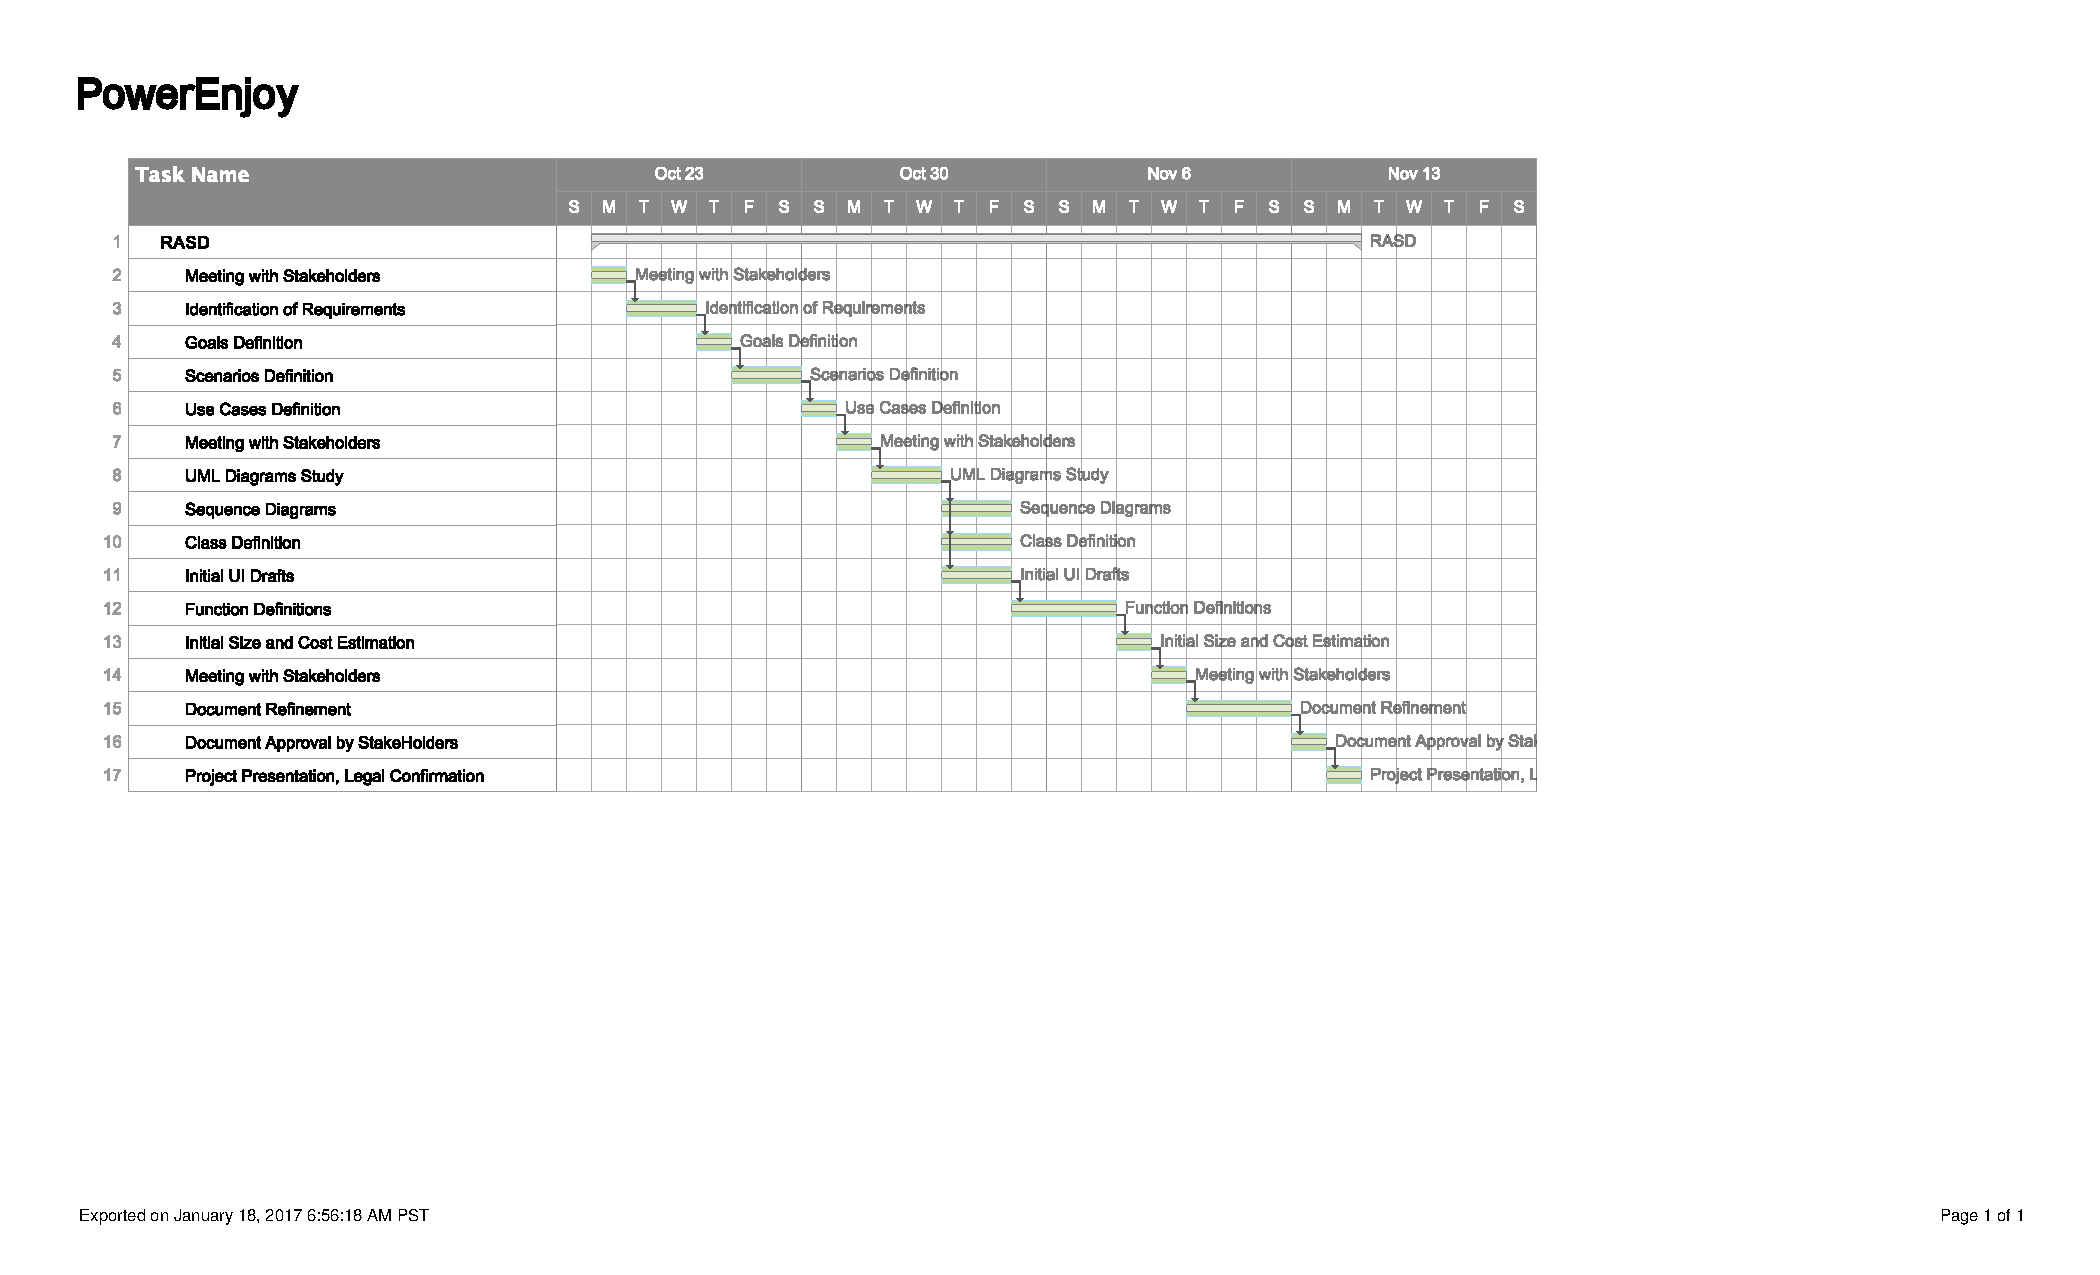
\includegraphics[width=1.5\textwidth]{RASD_Schedule.png}}%
\vspace*{0cm}
\end{figure}
\begin{figure}[h]
\centering
\vspace*{\fill}
\noindent\makebox[\textwidth]{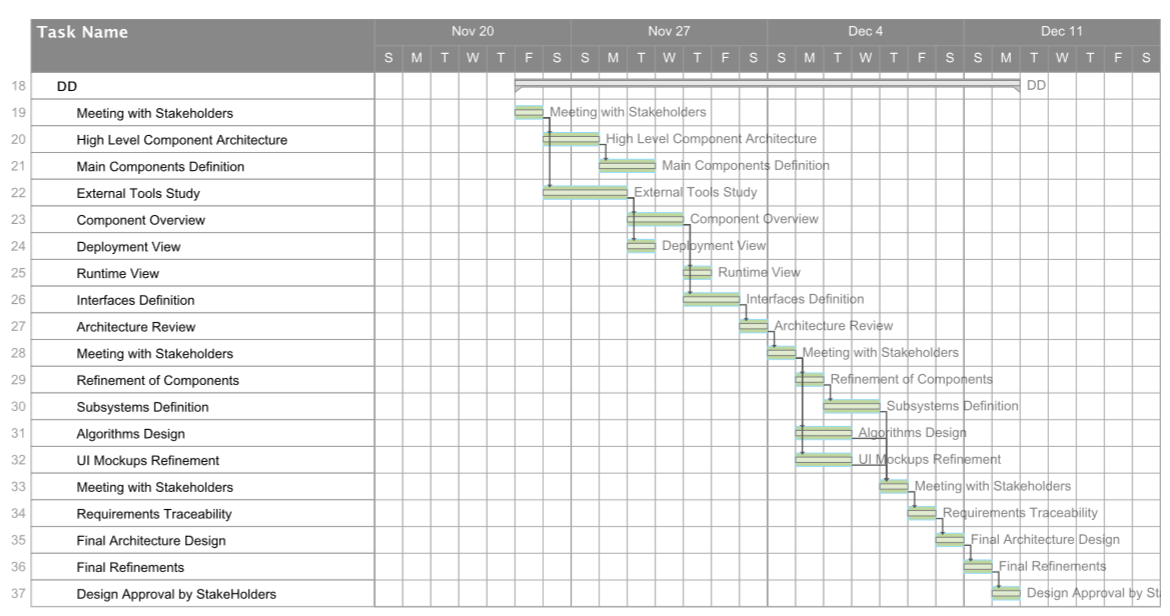
\includegraphics[width=1.42\textwidth]{DD_Schedule.png}}%
\vspace*{0cm}
\end{figure}
\begin{figure}[h]
\centering
\vspace*{\fill}
\noindent\makebox[\textwidth]{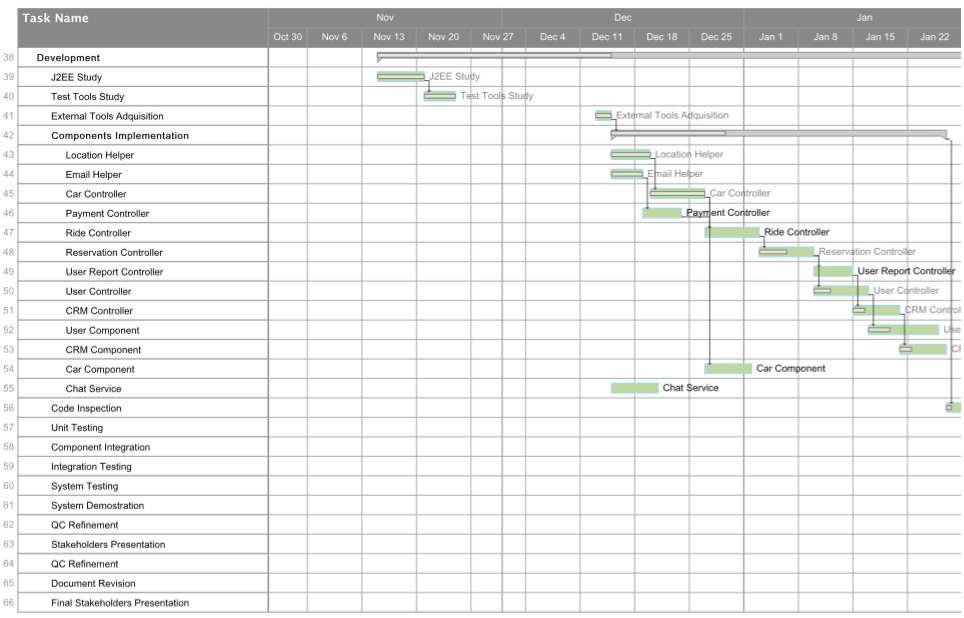
\includegraphics[width=1.42\textwidth]{Dev_Schedule1.png}}%
\vspace*{0.5cm}
\end{figure}
\begin{figure}[h]
\centering
\vspace*{\fill}
\noindent\makebox[\textwidth]{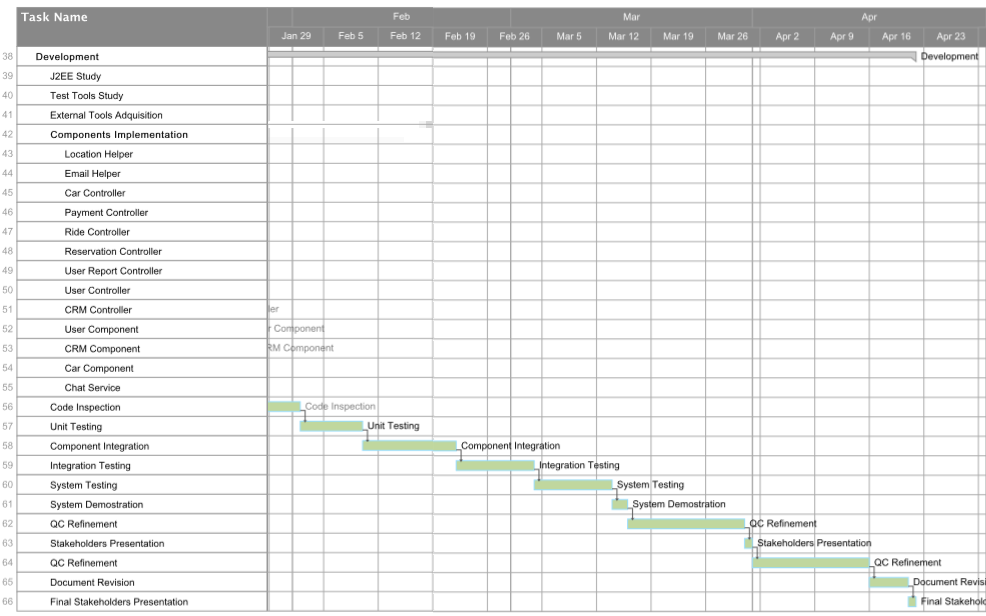
\includegraphics[width=1.5\textwidth]{Dev_Schedule2.png}}%
\vspace*{0.5cm}
\end{figure}
\begin{figure}[h]
\centering
\vspace*{\fill}
\noindent\makebox[\textwidth]{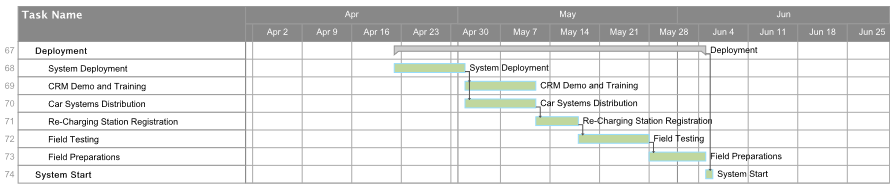
\includegraphics[width=1.5\textwidth]{Deployment_Schedule.png}}%
\vspace*{0.5cm}
\end{figure}

\section{Resource Allocation}
\section{Risk Management}

\newpage
\section{Effort Spent}
\begin{tabular}{ | c | c | c | c | }
\hline
	\textbf {Date} & \textbf {Domenico} & \textbf {Caio} & \textbf {Matheus} \\ \hline
	15/01/17& 2h & 2h & 2h  \\ \hline
	16/01/17& - & - & - \\ \hline
	17/01/17& 4h & - & - \\ \hline
	18/01/17& 4h & - & - \\ \hline
	19/01/17& - & 6h & - \\ \hline
	20/01/17& - & - & - \\ \hline
	21/01/17& - & - & - \\ \hline
	22/01/17& - & - & - \\ \hline
\end{tabular}
\newpage

\section{Changelog}
As the project and design decisions may change during the development this document is also prone to change.
We'll document every version in this part.
\begin{itemize}
\item \textbf {Version 1.1:} 22/01/2017
\end{itemize}
\end{document}
